\documentclass[../2.tex]{subfiles}
\begin{document}

We now proceed by analogy with the previous section and define a \ii{discrete Dirichlet energy} on graphs, using the laplacian matrix written on the canonical basis, as
in definition \ref{lapdef}.

\begin{defn}
    Let $A,\Phi$ be to $n\times n$ matrices, we define the \ii{discrete Dirichlet energy} to be 
    \[ D[\Phi] = \tr(\Phi^T \Delta \Phi). \]
\end{defn}

The minimization of the discrete Dirichlet energy is not a variational problem, rather a simple minimization in $\Phi$ in which we can 
use the standard Lagrange multipliers theorem. Here the $0$-laplacian is a matrix instead of a differential operator. The analogies between
this matrix and the differential operator is due to the chain complex structure.

\begin{prop}
    The minimum for the Dirichlet energy $ \tr(\Phi^T \Delta \Phi)$ constrained to the $\Phi$ such that $\Phi^T \Phi = 1$ is reached when the
    rows of $\Phi$ are the laplacian eigenvectors.
\end{prop}
\begin{proof}
    The constrained action can also be written as
    \[ D[\Phi] = \sum_{i,j,k} \Phi_{ik} \Delta_{ij} \Phi_{jk} - \sum_{i,j,k} \Lambda_{ij} \Phi_{kj} \Phi_{ki}, \]
    where $\Lambda$ is a diagonal matrix with the Lagrange multipliers as eigenvalues.\\ We then minimize this action 
    \[ \frac{\del D[\Phi]}{\del \Phi_{mn}} = \sum_{i,j,k} \delta_{im}\delta_{nk}\Delta_{ij} \Phi_{jk} + \sum_{i,j,k} \Phi_{ik} \Delta_{ij}\delta_{jm}\delta_{nk}
    - \sum_{i,j,k} \Lambda_{ij} \delta_{mk}\delta_{nj}\Phi_{ki} - \sum_{i,j,k} \Lambda_{ij} \Phi_{kj} \delta_{mk}\delta_{ni} =  \]
    \[ = \sum_{j} \Delta_{mj} \Phi_{jn} + \sum_{i} \Phi_{in} \Delta_{im} - \sum_{i} \Lambda_{in} \Phi_{mi} - \sum_{j} \Lambda_{nj} \Phi_{mj} = 0, \]
    which using the symmetry of $\Lambda$ and $A$ can be written as
    \[ \sum_{j} \Delta_{mj} \Phi_{jn} + \sum_{i}  \Delta_{mi} \Phi_{in} - \sum_{i} \Phi_{mi}\Lambda_{in} - \sum_{j} \Phi_{mj} \Lambda_{jn} =  \]
    \[ 2\Delta\Phi - 2\Phi\Lambda = 0. \]
    We then obtain 
    \[ \Delta\Phi = \Phi\Lambda, \]
    which for every row of $\Phi$ is an eigenvalue equation. \qedhere
\end{proof}

\begin{figure}[H]
    \centering
    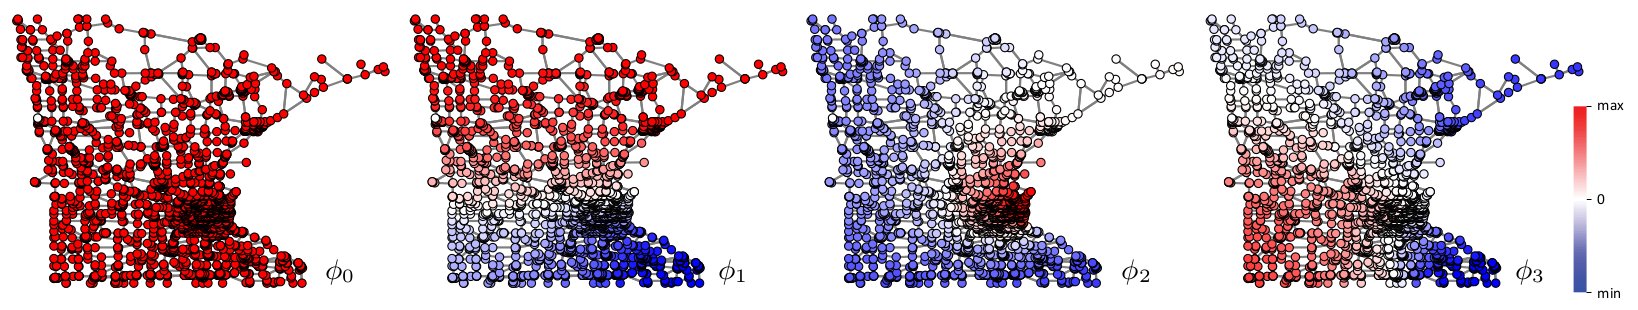
\includegraphics[width=17cm, height=4cm]{sections/2/eiglap}
    \caption{A graphical representation of the first laplacian eigenchains.}
    \label{fig:2:5}
\end{figure}

In figure \ref{fig:2:5} we can see some of the $0$-laplacian eigenfunctions. We notice that the eigenfunction corresponding to the eigenvalue $0$ is uniform as expected 
Eckmann's theorem for any connected component of the graph.

    
\end{document}